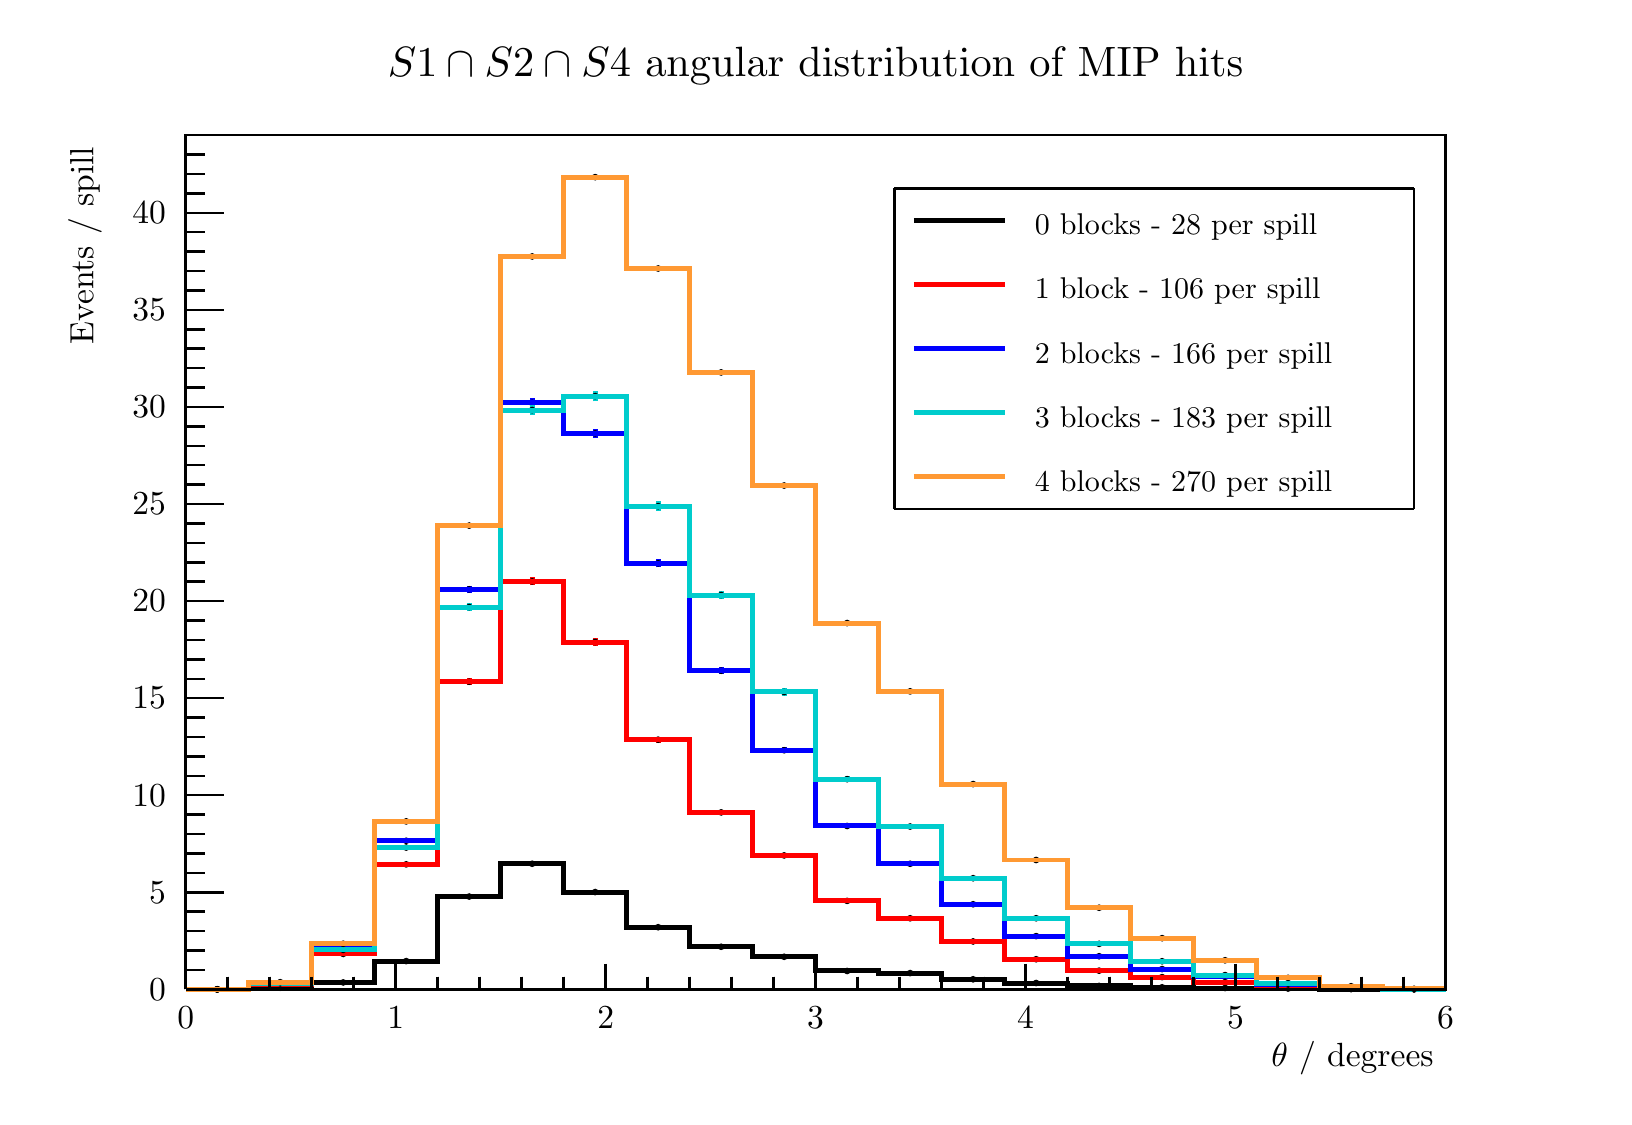
\begin{tikzpicture}
\pgfdeclareplotmark{cross} {
\pgfpathmoveto{\pgfpoint{-0.3\pgfplotmarksize}{\pgfplotmarksize}}
\pgfpathlineto{\pgfpoint{+0.3\pgfplotmarksize}{\pgfplotmarksize}}
\pgfpathlineto{\pgfpoint{+0.3\pgfplotmarksize}{0.3\pgfplotmarksize}}
\pgfpathlineto{\pgfpoint{+1\pgfplotmarksize}{0.3\pgfplotmarksize}}
\pgfpathlineto{\pgfpoint{+1\pgfplotmarksize}{-0.3\pgfplotmarksize}}
\pgfpathlineto{\pgfpoint{+0.3\pgfplotmarksize}{-0.3\pgfplotmarksize}}
\pgfpathlineto{\pgfpoint{+0.3\pgfplotmarksize}{-1.\pgfplotmarksize}}
\pgfpathlineto{\pgfpoint{-0.3\pgfplotmarksize}{-1.\pgfplotmarksize}}
\pgfpathlineto{\pgfpoint{-0.3\pgfplotmarksize}{-0.3\pgfplotmarksize}}
\pgfpathlineto{\pgfpoint{-1.\pgfplotmarksize}{-0.3\pgfplotmarksize}}
\pgfpathlineto{\pgfpoint{-1.\pgfplotmarksize}{0.3\pgfplotmarksize}}
\pgfpathlineto{\pgfpoint{-0.3\pgfplotmarksize}{0.3\pgfplotmarksize}}
\pgfpathclose
\pgfusepathqstroke
}
\pgfdeclareplotmark{cross*} {
\pgfpathmoveto{\pgfpoint{-0.3\pgfplotmarksize}{\pgfplotmarksize}}
\pgfpathlineto{\pgfpoint{+0.3\pgfplotmarksize}{\pgfplotmarksize}}
\pgfpathlineto{\pgfpoint{+0.3\pgfplotmarksize}{0.3\pgfplotmarksize}}
\pgfpathlineto{\pgfpoint{+1\pgfplotmarksize}{0.3\pgfplotmarksize}}
\pgfpathlineto{\pgfpoint{+1\pgfplotmarksize}{-0.3\pgfplotmarksize}}
\pgfpathlineto{\pgfpoint{+0.3\pgfplotmarksize}{-0.3\pgfplotmarksize}}
\pgfpathlineto{\pgfpoint{+0.3\pgfplotmarksize}{-1.\pgfplotmarksize}}
\pgfpathlineto{\pgfpoint{-0.3\pgfplotmarksize}{-1.\pgfplotmarksize}}
\pgfpathlineto{\pgfpoint{-0.3\pgfplotmarksize}{-0.3\pgfplotmarksize}}
\pgfpathlineto{\pgfpoint{-1.\pgfplotmarksize}{-0.3\pgfplotmarksize}}
\pgfpathlineto{\pgfpoint{-1.\pgfplotmarksize}{0.3\pgfplotmarksize}}
\pgfpathlineto{\pgfpoint{-0.3\pgfplotmarksize}{0.3\pgfplotmarksize}}
\pgfpathclose
\pgfusepathqfillstroke
}
\pgfdeclareplotmark{newstar} {
\pgfpathmoveto{\pgfqpoint{0pt}{\pgfplotmarksize}}
\pgfpathlineto{\pgfqpointpolar{44}{0.5\pgfplotmarksize}}
\pgfpathlineto{\pgfqpointpolar{18}{\pgfplotmarksize}}
\pgfpathlineto{\pgfqpointpolar{-20}{0.5\pgfplotmarksize}}
\pgfpathlineto{\pgfqpointpolar{-54}{\pgfplotmarksize}}
\pgfpathlineto{\pgfqpointpolar{-90}{0.5\pgfplotmarksize}}
\pgfpathlineto{\pgfqpointpolar{234}{\pgfplotmarksize}}
\pgfpathlineto{\pgfqpointpolar{198}{0.5\pgfplotmarksize}}
\pgfpathlineto{\pgfqpointpolar{162}{\pgfplotmarksize}}
\pgfpathlineto{\pgfqpointpolar{134}{0.5\pgfplotmarksize}}
\pgfpathclose
\pgfusepathqstroke
}
\pgfdeclareplotmark{newstar*} {
\pgfpathmoveto{\pgfqpoint{0pt}{\pgfplotmarksize}}
\pgfpathlineto{\pgfqpointpolar{44}{0.5\pgfplotmarksize}}
\pgfpathlineto{\pgfqpointpolar{18}{\pgfplotmarksize}}
\pgfpathlineto{\pgfqpointpolar{-20}{0.5\pgfplotmarksize}}
\pgfpathlineto{\pgfqpointpolar{-54}{\pgfplotmarksize}}
\pgfpathlineto{\pgfqpointpolar{-90}{0.5\pgfplotmarksize}}
\pgfpathlineto{\pgfqpointpolar{234}{\pgfplotmarksize}}
\pgfpathlineto{\pgfqpointpolar{198}{0.5\pgfplotmarksize}}
\pgfpathlineto{\pgfqpointpolar{162}{\pgfplotmarksize}}
\pgfpathlineto{\pgfqpointpolar{134}{0.5\pgfplotmarksize}}
\pgfpathclose
\pgfusepathqfillstroke
}
\definecolor{c}{rgb}{1,1,1};
\draw [color=c, fill=c] (0,0) rectangle (20,13.5632);
\draw [color=c, fill=c] (2,1.35632) rectangle (18,12.2069);
\definecolor{c}{rgb}{0,0,0};
\draw [c,line width=0.9] (2,1.35632) -- (2,12.2069) -- (18,12.2069) -- (18,1.35632) -- (2,1.35632);
\definecolor{c}{rgb}{1,1,1};
\draw [color=c, fill=c] (2,1.35632) rectangle (18,12.2069);
\definecolor{c}{rgb}{0,0,0};
\draw [c,line width=0.9] (2,1.35632) -- (2,12.2069) -- (18,12.2069) -- (18,1.35632) -- (2,1.35632);
\definecolor{c}{rgb}{0,0,0.6};
\draw [c,line width=0.9] (2,1.35632) -- (2.8,1.35632) -- (2.8,1.35632) -- (3.6,1.35632) -- (3.6,1.35632) -- (4.4,1.35632) -- (4.4,1.35632) -- (5.2,1.35632) -- (5.2,1.35632) -- (6,1.35632) -- (6,1.35632) -- (6.8,1.35632) -- (6.8,1.35632) --
 (7.6,1.35632) -- (7.6,1.35632) -- (8.4,1.35632) -- (8.4,1.35632) -- (9.2,1.35632) -- (9.2,1.35632) -- (10,1.35632) -- (10,1.35632) -- (10.8,1.35632) -- (10.8,1.35632) -- (11.6,1.35632) -- (11.6,1.35632) -- (12.4,1.35632) -- (12.4,1.35632) --
 (13.2,1.35632) -- (13.2,1.35632) -- (14,1.35632) -- (14,1.35632) -- (14.8,1.35632) -- (14.8,1.35632) -- (15.6,1.35632) -- (15.6,1.35632) -- (16.4,1.35632) -- (16.4,1.35632) -- (17.2,1.35632) -- (17.2,1.35632) -- (18,1.35632);
\definecolor{c}{rgb}{0,0,0};
\draw [c,line width=0.9] (2,1.35632) -- (18,1.35632);
\draw [anchor= east] (18,0.488276) node[scale=1.2126, color=c, rotate=0]{$\theta$ / degrees};
\draw [c,line width=0.9] (2,1.68184) -- (2,1.35632);
\draw [c,line width=0.9] (2.53333,1.51908) -- (2.53333,1.35632);
\draw [c,line width=0.9] (3.06667,1.51908) -- (3.06667,1.35632);
\draw [c,line width=0.9] (3.6,1.51908) -- (3.6,1.35632);
\draw [c,line width=0.9] (4.13333,1.51908) -- (4.13333,1.35632);
\draw [c,line width=0.9] (4.66667,1.68184) -- (4.66667,1.35632);
\draw [c,line width=0.9] (5.2,1.51908) -- (5.2,1.35632);
\draw [c,line width=0.9] (5.73333,1.51908) -- (5.73333,1.35632);
\draw [c,line width=0.9] (6.26667,1.51908) -- (6.26667,1.35632);
\draw [c,line width=0.9] (6.8,1.51908) -- (6.8,1.35632);
\draw [c,line width=0.9] (7.33333,1.68184) -- (7.33333,1.35632);
\draw [c,line width=0.9] (7.86667,1.51908) -- (7.86667,1.35632);
\draw [c,line width=0.9] (8.4,1.51908) -- (8.4,1.35632);
\draw [c,line width=0.9] (8.93333,1.51908) -- (8.93333,1.35632);
\draw [c,line width=0.9] (9.46667,1.51908) -- (9.46667,1.35632);
\draw [c,line width=0.9] (10,1.68184) -- (10,1.35632);
\draw [c,line width=0.9] (10.5333,1.51908) -- (10.5333,1.35632);
\draw [c,line width=0.9] (11.0667,1.51908) -- (11.0667,1.35632);
\draw [c,line width=0.9] (11.6,1.51908) -- (11.6,1.35632);
\draw [c,line width=0.9] (12.1333,1.51908) -- (12.1333,1.35632);
\draw [c,line width=0.9] (12.6667,1.68184) -- (12.6667,1.35632);
\draw [c,line width=0.9] (13.2,1.51908) -- (13.2,1.35632);
\draw [c,line width=0.9] (13.7333,1.51908) -- (13.7333,1.35632);
\draw [c,line width=0.9] (14.2667,1.51908) -- (14.2667,1.35632);
\draw [c,line width=0.9] (14.8,1.51908) -- (14.8,1.35632);
\draw [c,line width=0.9] (15.3333,1.68184) -- (15.3333,1.35632);
\draw [c,line width=0.9] (15.8667,1.51908) -- (15.8667,1.35632);
\draw [c,line width=0.9] (16.4,1.51908) -- (16.4,1.35632);
\draw [c,line width=0.9] (16.9333,1.51908) -- (16.9333,1.35632);
\draw [c,line width=0.9] (17.4667,1.51908) -- (17.4667,1.35632);
\draw [c,line width=0.9] (18,1.68184) -- (18,1.35632);
\draw [anchor=base] (2,0.854483) node[scale=1.2126, color=c, rotate=0]{0};
\draw [anchor=base] (4.66667,0.854483) node[scale=1.2126, color=c, rotate=0]{1};
\draw [anchor=base] (7.33333,0.854483) node[scale=1.2126, color=c, rotate=0]{2};
\draw [anchor=base] (10,0.854483) node[scale=1.2126, color=c, rotate=0]{3};
\draw [anchor=base] (12.6667,0.854483) node[scale=1.2126, color=c, rotate=0]{4};
\draw [anchor=base] (15.3333,0.854483) node[scale=1.2126, color=c, rotate=0]{5};
\draw [anchor=base] (18,0.854483) node[scale=1.2126, color=c, rotate=0]{6};
\draw [c,line width=0.9] (2,1.35632) -- (2,12.2069);
\draw [anchor= east] (0.72,12.2069) node[scale=1.2126, color=c, rotate=90]{ Events / spill};
\draw [c,line width=0.9] (2.48,1.35632) -- (2,1.35632);
\draw [c,line width=0.9] (2.24,1.60289) -- (2,1.60289);
\draw [c,line width=0.9] (2.24,1.84945) -- (2,1.84945);
\draw [c,line width=0.9] (2.24,2.09602) -- (2,2.09602);
\draw [c,line width=0.9] (2.24,2.34258) -- (2,2.34258);
\draw [c,line width=0.9] (2.48,2.58915) -- (2,2.58915);
\draw [c,line width=0.9] (2.24,2.83571) -- (2,2.83571);
\draw [c,line width=0.9] (2.24,3.08228) -- (2,3.08228);
\draw [c,line width=0.9] (2.24,3.32884) -- (2,3.32884);
\draw [c,line width=0.9] (2.24,3.57541) -- (2,3.57541);
\draw [c,line width=0.9] (2.48,3.82197) -- (2,3.82197);
\draw [c,line width=0.9] (2.24,4.06854) -- (2,4.06854);
\draw [c,line width=0.9] (2.24,4.31511) -- (2,4.31511);
\draw [c,line width=0.9] (2.24,4.56167) -- (2,4.56167);
\draw [c,line width=0.9] (2.24,4.80824) -- (2,4.80824);
\draw [c,line width=0.9] (2.48,5.0548) -- (2,5.0548);
\draw [c,line width=0.9] (2.24,5.30137) -- (2,5.30137);
\draw [c,line width=0.9] (2.24,5.54793) -- (2,5.54793);
\draw [c,line width=0.9] (2.24,5.7945) -- (2,5.7945);
\draw [c,line width=0.9] (2.24,6.04106) -- (2,6.04106);
\draw [c,line width=0.9] (2.48,6.28763) -- (2,6.28763);
\draw [c,line width=0.9] (2.24,6.53419) -- (2,6.53419);
\draw [c,line width=0.9] (2.24,6.78076) -- (2,6.78076);
\draw [c,line width=0.9] (2.24,7.02732) -- (2,7.02732);
\draw [c,line width=0.9] (2.24,7.27389) -- (2,7.27389);
\draw [c,line width=0.9] (2.48,7.52045) -- (2,7.52045);
\draw [c,line width=0.9] (2.24,7.76702) -- (2,7.76702);
\draw [c,line width=0.9] (2.24,8.01359) -- (2,8.01359);
\draw [c,line width=0.9] (2.24,8.26015) -- (2,8.26015);
\draw [c,line width=0.9] (2.24,8.50672) -- (2,8.50672);
\draw [c,line width=0.9] (2.48,8.75328) -- (2,8.75328);
\draw [c,line width=0.9] (2.24,8.99985) -- (2,8.99985);
\draw [c,line width=0.9] (2.24,9.24641) -- (2,9.24641);
\draw [c,line width=0.9] (2.24,9.49298) -- (2,9.49298);
\draw [c,line width=0.9] (2.24,9.73954) -- (2,9.73954);
\draw [c,line width=0.9] (2.48,9.98611) -- (2,9.98611);
\draw [c,line width=0.9] (2.24,10.2327) -- (2,10.2327);
\draw [c,line width=0.9] (2.24,10.4792) -- (2,10.4792);
\draw [c,line width=0.9] (2.24,10.7258) -- (2,10.7258);
\draw [c,line width=0.9] (2.24,10.9724) -- (2,10.9724);
\draw [c,line width=0.9] (2.48,11.2189) -- (2,11.2189);
\draw [c,line width=0.9] (2.48,11.2189) -- (2,11.2189);
\draw [c,line width=0.9] (2.24,11.4655) -- (2,11.4655);
\draw [c,line width=0.9] (2.24,11.7121) -- (2,11.7121);
\draw [c,line width=0.9] (2.24,11.9586) -- (2,11.9586);
\draw [c,line width=0.9] (2.24,12.2052) -- (2,12.2052);
\draw [anchor= east] (1.9,1.35632) node[scale=1.2126, color=c, rotate=0]{0};
\draw [anchor= east] (1.9,2.58915) node[scale=1.2126, color=c, rotate=0]{5};
\draw [anchor= east] (1.9,3.82197) node[scale=1.2126, color=c, rotate=0]{10};
\draw [anchor= east] (1.9,5.0548) node[scale=1.2126, color=c, rotate=0]{15};
\draw [anchor= east] (1.9,6.28763) node[scale=1.2126, color=c, rotate=0]{20};
\draw [anchor= east] (1.9,7.52045) node[scale=1.2126, color=c, rotate=0]{25};
\draw [anchor= east] (1.9,8.75328) node[scale=1.2126, color=c, rotate=0]{30};
\draw [anchor= east] (1.9,9.98611) node[scale=1.2126, color=c, rotate=0]{35};
\draw [anchor= east] (1.9,11.2189) node[scale=1.2126, color=c, rotate=0]{40};
\draw [c,line width=1.8] (2.4,1.35632) -- (2.4,1.35667);
\draw [c,line width=1.8] (2.4,1.35667) -- (2.4,1.35701);
\foreach \P in {(2.4,1.35667)}{\draw[mark options={color=c,fill=c},mark size=2.402402pt,mark=*,mark size=1pt] plot coordinates {\P};}
\draw [c,line width=1.8] (3.2,1.37421) -- (3.2,1.37732);
\draw [c,line width=1.8] (3.2,1.37732) -- (3.2,1.38043);
\foreach \P in {(3.2,1.37732)}{\draw[mark options={color=c,fill=c},mark size=2.402402pt,mark=*,mark size=1pt] plot coordinates {\P};}
\draw [c,line width=1.8] (4,1.43826) -- (4,1.44474);
\draw [c,line width=1.8] (4,1.44474) -- (4,1.45123);
\foreach \P in {(4,1.44474)}{\draw[mark options={color=c,fill=c},mark size=2.402402pt,mark=*,mark size=1pt] plot coordinates {\P};}
\draw [c,line width=1.8] (4.8,1.70111) -- (4.8,1.71559);
\draw [c,line width=1.8] (4.8,1.71559) -- (4.8,1.73006);
\foreach \P in {(4.8,1.71559)}{\draw[mark options={color=c,fill=c},mark size=2.402402pt,mark=*,mark size=1pt] plot coordinates {\P};}
\draw [c,line width=1.8] (5.6,2.50801) -- (5.6,2.53547);
\draw [c,line width=1.8] (5.6,2.53547) -- (5.6,2.56293);
\foreach \P in {(5.6,2.53547)}{\draw[mark options={color=c,fill=c},mark size=2.402402pt,mark=*,mark size=1pt] plot coordinates {\P};}
\draw [c,line width=1.8] (6.4,2.91977) -- (6.4,2.95217);
\draw [c,line width=1.8] (6.4,2.95217) -- (6.4,2.98457);
\foreach \P in {(6.4,2.95217)}{\draw[mark options={color=c,fill=c},mark size=2.402402pt,mark=*,mark size=1pt] plot coordinates {\P};}
\draw [c,line width=1.8] (7.2,2.56376) -- (7.2,2.59229);
\draw [c,line width=1.8] (7.2,2.59229) -- (7.2,2.62081);
\foreach \P in {(7.2,2.59229)}{\draw[mark options={color=c,fill=c},mark size=2.402402pt,mark=*,mark size=1pt] plot coordinates {\P};}
\draw [c,line width=1.8] (8,2.12349) -- (8,2.14597);
\draw [c,line width=1.8] (8,2.14597) -- (8,2.16846);
\foreach \P in {(8,2.14597)}{\draw[mark options={color=c,fill=c},mark size=2.402402pt,mark=*,mark size=1pt] plot coordinates {\P};}
\draw [c,line width=1.8] (8.8,1.87945) -- (8.8,1.89768);
\draw [c,line width=1.8] (8.8,1.89768) -- (8.8,1.91591);
\foreach \P in {(8.8,1.89768)}{\draw[mark options={color=c,fill=c},mark size=2.402402pt,mark=*,mark size=1pt] plot coordinates {\P};}
\draw [c,line width=1.8] (9.6,1.75482) -- (9.6,1.77052);
\draw [c,line width=1.8] (9.6,1.77052) -- (9.6,1.78623);
\foreach \P in {(9.6,1.77052)}{\draw[mark options={color=c,fill=c},mark size=2.402402pt,mark=*,mark size=1pt] plot coordinates {\P};}
\draw [c,line width=1.8] (10.4,1.57888) -- (10.4,1.59008);
\draw [c,line width=1.8] (10.4,1.59008) -- (10.4,1.60128);
\foreach \P in {(10.4,1.59008)}{\draw[mark options={color=c,fill=c},mark size=2.402402pt,mark=*,mark size=1pt] plot coordinates {\P};}
\draw [c,line width=1.8] (11.2,1.55242) -- (11.2,1.56325);
\draw [c,line width=1.8] (11.2,1.56325) -- (11.2,1.57407);
\foreach \P in {(11.2,1.56325)}{\draw[mark options={color=c,fill=c},mark size=2.402402pt,mark=*,mark size=1pt] plot coordinates {\P};}
\draw [c,line width=1.8] (12,1.4762) -- (12,1.48457);
\draw [c,line width=1.8] (12,1.48457) -- (12,1.49294);
\foreach \P in {(12,1.48457)}{\draw[mark options={color=c,fill=c},mark size=2.402402pt,mark=*,mark size=1pt] plot coordinates {\P};}
\draw [c,line width=1.8] (12.8,1.43085) -- (12.8,1.43719);
\draw [c,line width=1.8] (12.8,1.43719) -- (12.8,1.44352);
\foreach \P in {(12.8,1.43719)}{\draw[mark options={color=c,fill=c},mark size=2.402402pt,mark=*,mark size=1pt] plot coordinates {\P};}
\draw [c,line width=1.8] (13.6,1.396) -- (13.6,1.40053);
\draw [c,line width=1.8] (13.6,1.40053) -- (13.6,1.40507);
\foreach \P in {(13.6,1.40053)}{\draw[mark options={color=c,fill=c},mark size=2.402402pt,mark=*,mark size=1pt] plot coordinates {\P};}
\draw [c,line width=1.8] (14.4,1.3793) -- (14.4,1.38292);
\draw [c,line width=1.8] (14.4,1.38292) -- (14.4,1.38654);
\foreach \P in {(14.4,1.38292)}{\draw[mark options={color=c,fill=c},mark size=2.402402pt,mark=*,mark size=1pt] plot coordinates {\P};}
\draw [c,line width=1.8] (15.2,1.37113) -- (15.2,1.37379);
\draw [c,line width=1.8] (15.2,1.37379) -- (15.2,1.37645);
\foreach \P in {(15.2,1.37379)}{\draw[mark options={color=c,fill=c},mark size=2.402402pt,mark=*,mark size=1pt] plot coordinates {\P};}
\draw [c,line width=1.8] (16,1.3653) -- (16,1.36731);
\draw [c,line width=1.8] (16,1.36731) -- (16,1.36933);
\foreach \P in {(16,1.36731)}{\draw[mark options={color=c,fill=c},mark size=2.402402pt,mark=*,mark size=1pt] plot coordinates {\P};}
\draw [c,line width=1.8] (16.8,1.35901) -- (16.8,1.36043);
\draw [c,line width=1.8] (16.8,1.36043) -- (16.8,1.36184);
\foreach \P in {(16.8,1.36043)}{\draw[mark options={color=c,fill=c},mark size=2.402402pt,mark=*,mark size=1pt] plot coordinates {\P};}
\draw [c,line width=1.8] (2,1.35632) -- (2.8,1.35632) -- (2.8,1.37732) -- (3.6,1.37732) -- (3.6,1.44474) -- (4.4,1.44474) -- (4.4,1.71559) -- (5.2,1.71559) -- (5.2,2.53547) -- (6,2.53547) -- (6,2.95217) -- (6.8,2.95217) -- (6.8,2.59229) --
 (7.6,2.59229) -- (7.6,2.14597) -- (8.4,2.14597) -- (8.4,1.89768) -- (9.2,1.89768) -- (9.2,1.77052) -- (10,1.77052) -- (10,1.59008) -- (10.8,1.59008) -- (10.8,1.56325) -- (11.6,1.56325) -- (11.6,1.48457) -- (12.4,1.48457) -- (12.4,1.43719) --
 (13.2,1.43719) -- (13.2,1.40053) -- (14,1.40053) -- (14,1.38292) -- (14.8,1.38292) -- (14.8,1.37379) -- (15.6,1.37379) -- (15.6,1.36731) -- (16.4,1.36731) -- (16.4,1.36043) -- (17.2,1.36043) -- (17.2,1.35632) -- (18,1.35632);
\definecolor{c}{rgb}{1,0,0};
\draw [c,line width=1.8] (2.4,1.35632) -- (2.4,1.35684);
\draw [c,line width=1.8] (2.4,1.35684) -- (2.4,1.35736);
\definecolor{c}{rgb}{0,0,0};
\foreach \P in {(2.4,1.35684)}{\draw[mark options={color=c,fill=c},mark size=2.402402pt,mark=*,mark size=1pt] plot coordinates {\P};}
\definecolor{c}{rgb}{1,0,0};
\draw [c,line width=1.8] (3.2,1.41399) -- (3.2,1.41942);
\draw [c,line width=1.8] (3.2,1.41942) -- (3.2,1.42485);
\definecolor{c}{rgb}{0,0,0};
\foreach \P in {(3.2,1.41942)}{\draw[mark options={color=c,fill=c},mark size=2.402402pt,mark=*,mark size=1pt] plot coordinates {\P};}
\definecolor{c}{rgb}{1,0,0};
\draw [c,line width=1.8] (4,1.79246) -- (4,1.8069);
\draw [c,line width=1.8] (4,1.8069) -- (4,1.82134);
\definecolor{c}{rgb}{0,0,0};
\foreach \P in {(4,1.8069)}{\draw[mark options={color=c,fill=c},mark size=2.402402pt,mark=*,mark size=1pt] plot coordinates {\P};}
\definecolor{c}{rgb}{1,0,0};
\draw [c,line width=1.8] (4.8,2.9168) -- (4.8,2.94435);
\draw [c,line width=1.8] (4.8,2.94435) -- (4.8,2.9719);
\definecolor{c}{rgb}{0,0,0};
\foreach \P in {(4.8,2.94435)}{\draw[mark options={color=c,fill=c},mark size=2.402402pt,mark=*,mark size=1pt] plot coordinates {\P};}
\definecolor{c}{rgb}{1,0,0};
\draw [c,line width=1.8] (5.6,5.21998) -- (5.6,5.26355);
\draw [c,line width=1.8] (5.6,5.26355) -- (5.6,5.30712);
\definecolor{c}{rgb}{0,0,0};
\foreach \P in {(5.6,5.26355)}{\draw[mark options={color=c,fill=c},mark size=2.402402pt,mark=*,mark size=1pt] plot coordinates {\P};}
\definecolor{c}{rgb}{1,0,0};
\draw [c,line width=1.8] (6.4,6.48763) -- (6.4,6.53825);
\draw [c,line width=1.8] (6.4,6.53825) -- (6.4,6.58887);
\definecolor{c}{rgb}{0,0,0};
\foreach \P in {(6.4,6.53825)}{\draw[mark options={color=c,fill=c},mark size=2.402402pt,mark=*,mark size=1pt] plot coordinates {\P};}
\definecolor{c}{rgb}{1,0,0};
\draw [c,line width=1.8] (7.2,5.7211) -- (7.2,5.76788);
\draw [c,line width=1.8] (7.2,5.76788) -- (7.2,5.81465);
\definecolor{c}{rgb}{0,0,0};
\foreach \P in {(7.2,5.76788)}{\draw[mark options={color=c,fill=c},mark size=2.402402pt,mark=*,mark size=1pt] plot coordinates {\P};}
\definecolor{c}{rgb}{1,0,0};
\draw [c,line width=1.8] (8,4.48824) -- (8,4.52785);
\draw [c,line width=1.8] (8,4.52785) -- (8,4.56745);
\definecolor{c}{rgb}{0,0,0};
\foreach \P in {(8,4.52785)}{\draw[mark options={color=c,fill=c},mark size=2.402402pt,mark=*,mark size=1pt] plot coordinates {\P};}
\definecolor{c}{rgb}{1,0,0};
\draw [c,line width=1.8] (8.8,3.57095) -- (8.8,3.60412);
\draw [c,line width=1.8] (8.8,3.60412) -- (8.8,3.63729);
\definecolor{c}{rgb}{0,0,0};
\foreach \P in {(8.8,3.60412)}{\draw[mark options={color=c,fill=c},mark size=2.402402pt,mark=*,mark size=1pt] plot coordinates {\P};}
\definecolor{c}{rgb}{1,0,0};
\draw [c,line width=1.8] (9.6,3.02904) -- (9.6,3.0578);
\draw [c,line width=1.8] (9.6,3.0578) -- (9.6,3.08655);
\definecolor{c}{rgb}{0,0,0};
\foreach \P in {(9.6,3.0578)}{\draw[mark options={color=c,fill=c},mark size=2.402402pt,mark=*,mark size=1pt] plot coordinates {\P};}
\definecolor{c}{rgb}{1,0,0};
\draw [c,line width=1.8] (10.4,2.45738) -- (10.4,2.48051);
\draw [c,line width=1.8] (10.4,2.48051) -- (10.4,2.50364);
\definecolor{c}{rgb}{0,0,0};
\foreach \P in {(10.4,2.48051)}{\draw[mark options={color=c,fill=c},mark size=2.402402pt,mark=*,mark size=1pt] plot coordinates {\P};}
\definecolor{c}{rgb}{1,0,0};
\draw [c,line width=1.8] (11.2,2.23876) -- (11.2,2.25958);
\draw [c,line width=1.8] (11.2,2.25958) -- (11.2,2.2804);
\definecolor{c}{rgb}{0,0,0};
\foreach \P in {(11.2,2.25958)}{\draw[mark options={color=c,fill=c},mark size=2.402402pt,mark=*,mark size=1pt] plot coordinates {\P};}
\definecolor{c}{rgb}{1,0,0};
\draw [c,line width=1.8] (12,1.9482) -- (12,1.96524);
\draw [c,line width=1.8] (12,1.96524) -- (12,1.98228);
\definecolor{c}{rgb}{0,0,0};
\foreach \P in {(12,1.96524)}{\draw[mark options={color=c,fill=c},mark size=2.402402pt,mark=*,mark size=1pt] plot coordinates {\P};}
\definecolor{c}{rgb}{1,0,0};
\draw [c,line width=1.8] (12.8,1.72599) -- (12.8,1.73946);
\draw [c,line width=1.8] (12.8,1.73946) -- (12.8,1.75293);
\definecolor{c}{rgb}{0,0,0};
\foreach \P in {(12.8,1.73946)}{\draw[mark options={color=c,fill=c},mark size=2.402402pt,mark=*,mark size=1pt] plot coordinates {\P};}
\definecolor{c}{rgb}{1,0,0};
\draw [c,line width=1.8] (13.6,1.58383) -- (13.6,1.59435);
\draw [c,line width=1.8] (13.6,1.59435) -- (13.6,1.60486);
\definecolor{c}{rgb}{0,0,0};
\foreach \P in {(13.6,1.59435)}{\draw[mark options={color=c,fill=c},mark size=2.402402pt,mark=*,mark size=1pt] plot coordinates {\P};}
\definecolor{c}{rgb}{1,0,0};
\draw [c,line width=1.8] (14.4,1.50365) -- (14.4,1.5122);
\draw [c,line width=1.8] (14.4,1.5122) -- (14.4,1.52075);
\definecolor{c}{rgb}{0,0,0};
\foreach \P in {(14.4,1.5122)}{\draw[mark options={color=c,fill=c},mark size=2.402402pt,mark=*,mark size=1pt] plot coordinates {\P};}
\definecolor{c}{rgb}{1,0,0};
\draw [c,line width=1.8] (15.2,1.44017) -- (15.2,1.44659);
\draw [c,line width=1.8] (15.2,1.44659) -- (15.2,1.45301);
\definecolor{c}{rgb}{0,0,0};
\foreach \P in {(15.2,1.44659)}{\draw[mark options={color=c,fill=c},mark size=2.402402pt,mark=*,mark size=1pt] plot coordinates {\P};}
\definecolor{c}{rgb}{1,0,0};
\draw [c,line width=1.8] (16,1.39317) -- (16,1.39741);
\draw [c,line width=1.8] (16,1.39741) -- (16,1.40165);
\definecolor{c}{rgb}{0,0,0};
\foreach \P in {(16,1.39741)}{\draw[mark options={color=c,fill=c},mark size=2.402402pt,mark=*,mark size=1pt] plot coordinates {\P};}
\definecolor{c}{rgb}{1,0,0};
\draw [c,line width=1.8] (16.8,1.36205) -- (16.8,1.36376);
\draw [c,line width=1.8] (16.8,1.36376) -- (16.8,1.36548);
\definecolor{c}{rgb}{0,0,0};
\foreach \P in {(16.8,1.36376)}{\draw[mark options={color=c,fill=c},mark size=2.402402pt,mark=*,mark size=1pt] plot coordinates {\P};}
\definecolor{c}{rgb}{1,0,0};
\draw [c,line width=1.8] (17.6,1.35734) -- (17.6,1.35821);
\draw [c,line width=1.8] (17.6,1.35821) -- (17.6,1.35909);
\definecolor{c}{rgb}{0,0,0};
\foreach \P in {(17.6,1.35821)}{\draw[mark options={color=c,fill=c},mark size=2.402402pt,mark=*,mark size=1pt] plot coordinates {\P};}
\definecolor{c}{rgb}{1,0,0};
\draw [c,line width=1.8] (2,1.35632) -- (2.8,1.35632) -- (2.8,1.41942) -- (3.6,1.41942) -- (3.6,1.8069) -- (4.4,1.8069) -- (4.4,2.94435) -- (5.2,2.94435) -- (5.2,5.26355) -- (6,5.26355) -- (6,6.53825) -- (6.8,6.53825) -- (6.8,5.76788) --
 (7.6,5.76788) -- (7.6,4.52785) -- (8.4,4.52785) -- (8.4,3.60412) -- (9.2,3.60412) -- (9.2,3.0578) -- (10,3.0578) -- (10,2.48051) -- (10.8,2.48051) -- (10.8,2.25958) -- (11.6,2.25958) -- (11.6,1.96524) -- (12.4,1.96524) -- (12.4,1.73946) --
 (13.2,1.73946) -- (13.2,1.59435) -- (14,1.59435) -- (14,1.5122) -- (14.8,1.5122) -- (14.8,1.44659) -- (15.6,1.44659) -- (15.6,1.39741) -- (16.4,1.39741) -- (16.4,1.36376) -- (17.2,1.36376) -- (17.2,1.35821) -- (18,1.35821);
\definecolor{c}{rgb}{0,0,1};
\draw [c,line width=1.8] (2.4,1.35708) -- (2.4,1.3579);
\draw [c,line width=1.8] (2.4,1.3579) -- (2.4,1.35872);
\definecolor{c}{rgb}{0,0,0};
\foreach \P in {(2.4,1.3579)}{\draw[mark options={color=c,fill=c},mark size=2.402402pt,mark=*,mark size=1pt] plot coordinates {\P};}
\definecolor{c}{rgb}{0,0,1};
\draw [c,line width=1.8] (3.2,1.4364) -- (3.2,1.44247);
\draw [c,line width=1.8] (3.2,1.44247) -- (3.2,1.44854);
\definecolor{c}{rgb}{0,0,0};
\foreach \P in {(3.2,1.44247)}{\draw[mark options={color=c,fill=c},mark size=2.402402pt,mark=*,mark size=1pt] plot coordinates {\P};}
\definecolor{c}{rgb}{0,0,1};
\draw [c,line width=1.8] (4,1.87947) -- (4,1.89447);
\draw [c,line width=1.8] (4,1.89447) -- (4,1.90948);
\definecolor{c}{rgb}{0,0,0};
\foreach \P in {(4,1.89447)}{\draw[mark options={color=c,fill=c},mark size=2.402402pt,mark=*,mark size=1pt] plot coordinates {\P};}
\definecolor{c}{rgb}{0,0,1};
\draw [c,line width=1.8] (4.8,3.21502) -- (4.8,3.24377);
\draw [c,line width=1.8] (4.8,3.24377) -- (4.8,3.27252);
\definecolor{c}{rgb}{0,0,0};
\foreach \P in {(4.8,3.24377)}{\draw[mark options={color=c,fill=c},mark size=2.402402pt,mark=*,mark size=1pt] plot coordinates {\P};}
\definecolor{c}{rgb}{0,0,1};
\draw [c,line width=1.8] (5.6,6.38923) -- (5.6,6.43726);
\draw [c,line width=1.8] (5.6,6.43726) -- (5.6,6.4853);
\definecolor{c}{rgb}{0,0,0};
\foreach \P in {(5.6,6.43726)}{\draw[mark options={color=c,fill=c},mark size=2.402402pt,mark=*,mark size=1pt] plot coordinates {\P};}
\definecolor{c}{rgb}{0,0,1};
\draw [c,line width=1.8] (6.4,8.74649) -- (6.4,8.80556);
\draw [c,line width=1.8] (6.4,8.80556) -- (6.4,8.86464);
\definecolor{c}{rgb}{0,0,0};
\foreach \P in {(6.4,8.80556)}{\draw[mark options={color=c,fill=c},mark size=2.402402pt,mark=*,mark size=1pt] plot coordinates {\P};}
\definecolor{c}{rgb}{0,0,1};
\draw [c,line width=1.8] (7.2,8.35944) -- (7.2,8.41733);
\draw [c,line width=1.8] (7.2,8.41733) -- (7.2,8.47523);
\definecolor{c}{rgb}{0,0,0};
\foreach \P in {(7.2,8.41733)}{\draw[mark options={color=c,fill=c},mark size=2.402402pt,mark=*,mark size=1pt] plot coordinates {\P};}
\definecolor{c}{rgb}{0,0,1};
\draw [c,line width=1.8] (8,6.71706) -- (8,6.76769);
\draw [c,line width=1.8] (8,6.76769) -- (8,6.81831);
\definecolor{c}{rgb}{0,0,0};
\foreach \P in {(8,6.76769)}{\draw[mark options={color=c,fill=c},mark size=2.402402pt,mark=*,mark size=1pt] plot coordinates {\P};}
\definecolor{c}{rgb}{0,0,1};
\draw [c,line width=1.8] (8.8,5.36035) -- (8.8,5.40382);
\draw [c,line width=1.8] (8.8,5.40382) -- (8.8,5.44729);
\definecolor{c}{rgb}{0,0,0};
\foreach \P in {(8.8,5.40382)}{\draw[mark options={color=c,fill=c},mark size=2.402402pt,mark=*,mark size=1pt] plot coordinates {\P};}
\definecolor{c}{rgb}{0,0,1};
\draw [c,line width=1.8] (9.6,4.35606) -- (9.6,4.39354);
\draw [c,line width=1.8] (9.6,4.39354) -- (9.6,4.43102);
\definecolor{c}{rgb}{0,0,0};
\foreach \P in {(9.6,4.39354)}{\draw[mark options={color=c,fill=c},mark size=2.402402pt,mark=*,mark size=1pt] plot coordinates {\P};}
\definecolor{c}{rgb}{0,0,1};
\draw [c,line width=1.8] (10.4,3.40078) -- (10.4,3.43159);
\draw [c,line width=1.8] (10.4,3.43159) -- (10.4,3.4624);
\definecolor{c}{rgb}{0,0,0};
\foreach \P in {(10.4,3.43159)}{\draw[mark options={color=c,fill=c},mark size=2.402402pt,mark=*,mark size=1pt] plot coordinates {\P};}
\definecolor{c}{rgb}{0,0,1};
\draw [c,line width=1.8] (11.2,2.92459) -- (11.2,2.95159);
\draw [c,line width=1.8] (11.2,2.95159) -- (11.2,2.9786);
\definecolor{c}{rgb}{0,0,0};
\foreach \P in {(11.2,2.95159)}{\draw[mark options={color=c,fill=c},mark size=2.402402pt,mark=*,mark size=1pt] plot coordinates {\P};}
\definecolor{c}{rgb}{0,0,1};
\draw [c,line width=1.8] (12,2.4153) -- (12,2.43751);
\draw [c,line width=1.8] (12,2.43751) -- (12,2.45973);
\definecolor{c}{rgb}{0,0,0};
\foreach \P in {(12,2.43751)}{\draw[mark options={color=c,fill=c},mark size=2.402402pt,mark=*,mark size=1pt] plot coordinates {\P};}
\definecolor{c}{rgb}{0,0,1};
\draw [c,line width=1.8] (12.8,2.01547) -- (12.8,2.03294);
\draw [c,line width=1.8] (12.8,2.03294) -- (12.8,2.05042);
\definecolor{c}{rgb}{0,0,0};
\foreach \P in {(12.8,2.03294)}{\draw[mark options={color=c,fill=c},mark size=2.402402pt,mark=*,mark size=1pt] plot coordinates {\P};}
\definecolor{c}{rgb}{0,0,1};
\draw [c,line width=1.8] (13.6,1.76361) -- (13.6,1.77737);
\draw [c,line width=1.8] (13.6,1.77737) -- (13.6,1.79112);
\definecolor{c}{rgb}{0,0,0};
\foreach \P in {(13.6,1.77737)}{\draw[mark options={color=c,fill=c},mark size=2.402402pt,mark=*,mark size=1pt] plot coordinates {\P};}
\definecolor{c}{rgb}{0,0,1};
\draw [c,line width=1.8] (14.4,1.6037) -- (14.4,1.61434);
\draw [c,line width=1.8] (14.4,1.61434) -- (14.4,1.62498);
\definecolor{c}{rgb}{0,0,0};
\foreach \P in {(14.4,1.61434)}{\draw[mark options={color=c,fill=c},mark size=2.402402pt,mark=*,mark size=1pt] plot coordinates {\P};}
\definecolor{c}{rgb}{0,0,1};
\draw [c,line width=1.8] (15.2,1.50924) -- (15.2,1.51757);
\draw [c,line width=1.8] (15.2,1.51757) -- (15.2,1.5259);
\definecolor{c}{rgb}{0,0,0};
\foreach \P in {(15.2,1.51757)}{\draw[mark options={color=c,fill=c},mark size=2.402402pt,mark=*,mark size=1pt] plot coordinates {\P};}
\definecolor{c}{rgb}{0,0,1};
\draw [c,line width=1.8] (16,1.41395) -- (16,1.41894);
\draw [c,line width=1.8] (16,1.41894) -- (16,1.42392);
\definecolor{c}{rgb}{0,0,0};
\foreach \P in {(16,1.41894)}{\draw[mark options={color=c,fill=c},mark size=2.402402pt,mark=*,mark size=1pt] plot coordinates {\P};}
\definecolor{c}{rgb}{0,0,1};
\draw [c,line width=1.8] (16.8,1.37118) -- (16.8,1.37369);
\draw [c,line width=1.8] (16.8,1.37369) -- (16.8,1.3762);
\definecolor{c}{rgb}{0,0,0};
\foreach \P in {(16.8,1.37369)}{\draw[mark options={color=c,fill=c},mark size=2.402402pt,mark=*,mark size=1pt] plot coordinates {\P};}
\definecolor{c}{rgb}{0,0,1};
\draw [c,line width=1.8] (17.6,1.35734) -- (17.6,1.35787);
\draw [c,line width=1.8] (17.6,1.35787) -- (17.6,1.3584);
\definecolor{c}{rgb}{0,0,0};
\foreach \P in {(17.6,1.35787)}{\draw[mark options={color=c,fill=c},mark size=2.402402pt,mark=*,mark size=1pt] plot coordinates {\P};}
\definecolor{c}{rgb}{0,0,1};
\draw [c,line width=1.8] (2,1.3579) -- (2.8,1.3579) -- (2.8,1.44247) -- (3.6,1.44247) -- (3.6,1.89447) -- (4.4,1.89447) -- (4.4,3.24377) -- (5.2,3.24377) -- (5.2,6.43726) -- (6,6.43726) -- (6,8.80556) -- (6.8,8.80556) -- (6.8,8.41733) --
 (7.6,8.41733) -- (7.6,6.76769) -- (8.4,6.76769) -- (8.4,5.40382) -- (9.2,5.40382) -- (9.2,4.39354) -- (10,4.39354) -- (10,3.43159) -- (10.8,3.43159) -- (10.8,2.95159) -- (11.6,2.95159) -- (11.6,2.43751) -- (12.4,2.43751) -- (12.4,2.03294) --
 (13.2,2.03294) -- (13.2,1.77737) -- (14,1.77737) -- (14,1.61434) -- (14.8,1.61434) -- (14.8,1.51757) -- (15.6,1.51757) -- (15.6,1.41894) -- (16.4,1.41894) -- (16.4,1.37369) -- (17.2,1.37369) -- (17.2,1.35787) -- (18,1.35787);
\definecolor{c}{rgb}{0,0.8,0.8};
\draw [c,line width=1.8] (2.4,1.35646) -- (2.4,1.3568);
\draw [c,line width=1.8] (2.4,1.3568) -- (2.4,1.35714);
\definecolor{c}{rgb}{0,0,0};
\foreach \P in {(2.4,1.3568)}{\draw[mark options={color=c,fill=c},mark size=2.402402pt,mark=*,mark size=1pt] plot coordinates {\P};}
\definecolor{c}{rgb}{0,0.8,0.8};
\draw [c,line width=1.8] (3.2,1.42647) -- (3.2,1.43272);
\draw [c,line width=1.8] (3.2,1.43272) -- (3.2,1.43898);
\definecolor{c}{rgb}{0,0,0};
\foreach \P in {(3.2,1.43272)}{\draw[mark options={color=c,fill=c},mark size=2.402402pt,mark=*,mark size=1pt] plot coordinates {\P};}
\definecolor{c}{rgb}{0,0.8,0.8};
\draw [c,line width=1.8] (4,1.84302) -- (4,1.85912);
\draw [c,line width=1.8] (4,1.85912) -- (4,1.87522);
\definecolor{c}{rgb}{0,0,0};
\foreach \P in {(4,1.85912)}{\draw[mark options={color=c,fill=c},mark size=2.402402pt,mark=*,mark size=1pt] plot coordinates {\P};}
\definecolor{c}{rgb}{0,0.8,0.8};
\draw [c,line width=1.8] (4.8,3.1265) -- (4.8,3.15769);
\draw [c,line width=1.8] (4.8,3.15769) -- (4.8,3.18888);
\definecolor{c}{rgb}{0,0,0};
\foreach \P in {(4.8,3.15769)}{\draw[mark options={color=c,fill=c},mark size=2.402402pt,mark=*,mark size=1pt] plot coordinates {\P};}
\definecolor{c}{rgb}{0,0.8,0.8};
\draw [c,line width=1.8] (5.6,6.16038) -- (5.6,6.21228);
\draw [c,line width=1.8] (5.6,6.21228) -- (5.6,6.26419);
\definecolor{c}{rgb}{0,0,0};
\foreach \P in {(5.6,6.21228)}{\draw[mark options={color=c,fill=c},mark size=2.402402pt,mark=*,mark size=1pt] plot coordinates {\P};}
\definecolor{c}{rgb}{0,0.8,0.8};
\draw [c,line width=1.8] (6.4,8.64917) -- (6.4,8.71421);
\draw [c,line width=1.8] (6.4,8.71421) -- (6.4,8.77925);
\definecolor{c}{rgb}{0,0,0};
\foreach \P in {(6.4,8.71421)}{\draw[mark options={color=c,fill=c},mark size=2.402402pt,mark=*,mark size=1pt] plot coordinates {\P};}
\definecolor{c}{rgb}{0,0.8,0.8};
\draw [c,line width=1.8] (7.2,8.82499) -- (7.2,8.89116);
\draw [c,line width=1.8] (7.2,8.89116) -- (7.2,8.95733);
\definecolor{c}{rgb}{0,0,0};
\foreach \P in {(7.2,8.89116)}{\draw[mark options={color=c,fill=c},mark size=2.402402pt,mark=*,mark size=1pt] plot coordinates {\P};}
\definecolor{c}{rgb}{0,0.8,0.8};
\draw [c,line width=1.8] (8,7.43356) -- (8,7.49332);
\draw [c,line width=1.8] (8,7.49332) -- (8,7.55307);
\definecolor{c}{rgb}{0,0,0};
\foreach \P in {(8,7.49332)}{\draw[mark options={color=c,fill=c},mark size=2.402402pt,mark=*,mark size=1pt] plot coordinates {\P};}
\definecolor{c}{rgb}{0,0.8,0.8};
\draw [c,line width=1.8] (8.8,6.31114) -- (8.8,6.36475);
\draw [c,line width=1.8] (8.8,6.36475) -- (8.8,6.41837);
\definecolor{c}{rgb}{0,0,0};
\foreach \P in {(8.8,6.36475)}{\draw[mark options={color=c,fill=c},mark size=2.402402pt,mark=*,mark size=1pt] plot coordinates {\P};}
\definecolor{c}{rgb}{0,0.8,0.8};
\draw [c,line width=1.8] (9.6,5.08723) -- (9.6,5.13359);
\draw [c,line width=1.8] (9.6,5.13359) -- (9.6,5.17995);
\definecolor{c}{rgb}{0,0,0};
\foreach \P in {(9.6,5.13359)}{\draw[mark options={color=c,fill=c},mark size=2.402402pt,mark=*,mark size=1pt] plot coordinates {\P};}
\definecolor{c}{rgb}{0,0.8,0.8};
\draw [c,line width=1.8] (10.4,3.98763) -- (10.4,4.02638);
\draw [c,line width=1.8] (10.4,4.02638) -- (10.4,4.06513);
\definecolor{c}{rgb}{0,0,0};
\foreach \P in {(10.4,4.02638)}{\draw[mark options={color=c,fill=c},mark size=2.402402pt,mark=*,mark size=1pt] plot coordinates {\P};}
\definecolor{c}{rgb}{0,0.8,0.8};
\draw [c,line width=1.8] (11.2,3.39082) -- (11.2,3.42484);
\draw [c,line width=1.8] (11.2,3.42484) -- (11.2,3.45886);
\definecolor{c}{rgb}{0,0,0};
\foreach \P in {(11.2,3.42484)}{\draw[mark options={color=c,fill=c},mark size=2.402402pt,mark=*,mark size=1pt] plot coordinates {\P};}
\definecolor{c}{rgb}{0,0.8,0.8};
\draw [c,line width=1.8] (12,2.74023) -- (12,2.7685);
\draw [c,line width=1.8] (12,2.7685) -- (12,2.79677);
\definecolor{c}{rgb}{0,0,0};
\foreach \P in {(12,2.7685)}{\draw[mark options={color=c,fill=c},mark size=2.402402pt,mark=*,mark size=1pt] plot coordinates {\P};}
\definecolor{c}{rgb}{0,0.8,0.8};
\draw [c,line width=1.8] (12.8,2.23769) -- (12.8,2.26014);
\draw [c,line width=1.8] (12.8,2.26014) -- (12.8,2.28259);
\definecolor{c}{rgb}{0,0,0};
\foreach \P in {(12.8,2.26014)}{\draw[mark options={color=c,fill=c},mark size=2.402402pt,mark=*,mark size=1pt] plot coordinates {\P};}
\definecolor{c}{rgb}{0,0.8,0.8};
\draw [c,line width=1.8] (13.6,1.917) -- (13.6,1.93488);
\draw [c,line width=1.8] (13.6,1.93488) -- (13.6,1.95276);
\definecolor{c}{rgb}{0,0,0};
\foreach \P in {(13.6,1.93488)}{\draw[mark options={color=c,fill=c},mark size=2.402402pt,mark=*,mark size=1pt] plot coordinates {\P};}
\definecolor{c}{rgb}{0,0.8,0.8};
\draw [c,line width=1.8] (14.4,1.69968) -- (14.4,1.71368);
\draw [c,line width=1.8] (14.4,1.71368) -- (14.4,1.72769);
\definecolor{c}{rgb}{0,0,0};
\foreach \P in {(14.4,1.71368)}{\draw[mark options={color=c,fill=c},mark size=2.402402pt,mark=*,mark size=1pt] plot coordinates {\P};}
\definecolor{c}{rgb}{0,0.8,0.8};
\draw [c,line width=1.8] (15.2,1.52798) -- (15.2,1.53786);
\draw [c,line width=1.8] (15.2,1.53786) -- (15.2,1.54774);
\definecolor{c}{rgb}{0,0,0};
\foreach \P in {(15.2,1.53786)}{\draw[mark options={color=c,fill=c},mark size=2.402402pt,mark=*,mark size=1pt] plot coordinates {\P};}
\definecolor{c}{rgb}{0,0.8,0.8};
\draw [c,line width=1.8] (16,1.42415) -- (16,1.43026);
\draw [c,line width=1.8] (16,1.43026) -- (16,1.43636);
\definecolor{c}{rgb}{0,0,0};
\foreach \P in {(16,1.43026)}{\draw[mark options={color=c,fill=c},mark size=2.402402pt,mark=*,mark size=1pt] plot coordinates {\P};}
\definecolor{c}{rgb}{0,0.8,0.8};
\draw [c,line width=1.8] (16.8,1.36942) -- (16.8,1.37206);
\draw [c,line width=1.8] (16.8,1.37206) -- (16.8,1.3747);
\definecolor{c}{rgb}{0,0,0};
\foreach \P in {(16.8,1.37206)}{\draw[mark options={color=c,fill=c},mark size=2.402402pt,mark=*,mark size=1pt] plot coordinates {\P};}
\definecolor{c}{rgb}{0,0.8,0.8};
\draw [c,line width=1.8] (17.6,1.35831) -- (17.6,1.35934);
\draw [c,line width=1.8] (17.6,1.35934) -- (17.6,1.36037);
\definecolor{c}{rgb}{0,0,0};
\foreach \P in {(17.6,1.35934)}{\draw[mark options={color=c,fill=c},mark size=2.402402pt,mark=*,mark size=1pt] plot coordinates {\P};}
\definecolor{c}{rgb}{0,0.8,0.8};
\draw [c,line width=1.8] (2,1.35632) -- (2.8,1.35632) -- (2.8,1.43272) -- (3.6,1.43272) -- (3.6,1.85912) -- (4.4,1.85912) -- (4.4,3.15769) -- (5.2,3.15769) -- (5.2,6.21228) -- (6,6.21228) -- (6,8.71421) -- (6.8,8.71421) -- (6.8,8.89116) --
 (7.6,8.89116) -- (7.6,7.49332) -- (8.4,7.49332) -- (8.4,6.36475) -- (9.2,6.36475) -- (9.2,5.13359) -- (10,5.13359) -- (10,4.02638) -- (10.8,4.02638) -- (10.8,3.42484) -- (11.6,3.42484) -- (11.6,2.7685) -- (12.4,2.7685) -- (12.4,2.26014) --
 (13.2,2.26014) -- (13.2,1.93488) -- (14,1.93488) -- (14,1.71368) -- (14.8,1.71368) -- (14.8,1.53786) -- (15.6,1.53786) -- (15.6,1.43026) -- (16.4,1.43026) -- (16.4,1.37206) -- (17.2,1.37206) -- (17.2,1.35934) -- (18,1.35934);
\definecolor{c}{rgb}{1,0.6,0.2};
\draw [c,line width=1.8] (2.4,1.35673) -- (2.4,1.35686);
\draw [c,line width=1.8] (2.4,1.35686) -- (2.4,1.35698);
\definecolor{c}{rgb}{0,0,0};
\foreach \P in {(2.4,1.35686)}{\draw[mark options={color=c,fill=c},mark size=2.402402pt,mark=*,mark size=1pt] plot coordinates {\P};}
\definecolor{c}{rgb}{1,0.6,0.2};
\draw [c,line width=1.8] (3.2,1.44562) -- (3.2,1.44723);
\draw [c,line width=1.8] (3.2,1.44723) -- (3.2,1.44884);
\definecolor{c}{rgb}{0,0,0};
\foreach \P in {(3.2,1.44723)}{\draw[mark options={color=c,fill=c},mark size=2.402402pt,mark=*,mark size=1pt] plot coordinates {\P};}
\definecolor{c}{rgb}{1,0.6,0.2};
\draw [c,line width=1.8] (4,1.93205) -- (4,1.93611);
\draw [c,line width=1.8] (4,1.93611) -- (4,1.94018);
\definecolor{c}{rgb}{0,0,0};
\foreach \P in {(4,1.93611)}{\draw[mark options={color=c,fill=c},mark size=2.402402pt,mark=*,mark size=1pt] plot coordinates {\P};}
\definecolor{c}{rgb}{1,0.6,0.2};
\draw [c,line width=1.8] (4.8,3.48206) -- (4.8,3.49009);
\draw [c,line width=1.8] (4.8,3.49009) -- (4.8,3.49812);
\definecolor{c}{rgb}{0,0,0};
\foreach \P in {(4.8,3.49009)}{\draw[mark options={color=c,fill=c},mark size=2.402402pt,mark=*,mark size=1pt] plot coordinates {\P};}
\definecolor{c}{rgb}{1,0.6,0.2};
\draw [c,line width=1.8] (5.6,7.23314) -- (5.6,7.24674);
\draw [c,line width=1.8] (5.6,7.24674) -- (5.6,7.26034);
\definecolor{c}{rgb}{0,0,0};
\foreach \P in {(5.6,7.24674)}{\draw[mark options={color=c,fill=c},mark size=2.402402pt,mark=*,mark size=1pt] plot coordinates {\P};}
\definecolor{c}{rgb}{1,0.6,0.2};
\draw [c,line width=1.8] (6.4,10.6472) -- (6.4,10.6646);
\draw [c,line width=1.8] (6.4,10.6646) -- (6.4,10.682);
\definecolor{c}{rgb}{0,0,0};
\foreach \P in {(6.4,10.6646)}{\draw[mark options={color=c,fill=c},mark size=2.402402pt,mark=*,mark size=1pt] plot coordinates {\P};}
\definecolor{c}{rgb}{1,0.6,0.2};
\draw [c,line width=1.8] (7.2,11.6533) -- (7.2,11.6718);
\draw [c,line width=1.8] (7.2,11.6718) -- (7.2,11.6902);
\definecolor{c}{rgb}{0,0,0};
\foreach \P in {(7.2,11.6718)}{\draw[mark options={color=c,fill=c},mark size=2.402402pt,mark=*,mark size=1pt] plot coordinates {\P};}
\definecolor{c}{rgb}{1,0.6,0.2};
\draw [c,line width=1.8] (8,10.4942) -- (8,10.5116);
\draw [c,line width=1.8] (8,10.5116) -- (8,10.529);
\definecolor{c}{rgb}{0,0,0};
\foreach \P in {(8,10.5116)}{\draw[mark options={color=c,fill=c},mark size=2.402402pt,mark=*,mark size=1pt] plot coordinates {\P};}
\definecolor{c}{rgb}{1,0.6,0.2};
\draw [c,line width=1.8] (8.8,9.17579) -- (8.8,9.19177);
\draw [c,line width=1.8] (8.8,9.19177) -- (8.8,9.20775);
\definecolor{c}{rgb}{0,0,0};
\foreach \P in {(8.8,9.19177)}{\draw[mark options={color=c,fill=c},mark size=2.402402pt,mark=*,mark size=1pt] plot coordinates {\P};}
\definecolor{c}{rgb}{1,0.6,0.2};
\draw [c,line width=1.8] (9.6,7.74107) -- (9.6,7.75546);
\draw [c,line width=1.8] (9.6,7.75546) -- (9.6,7.76984);
\definecolor{c}{rgb}{0,0,0};
\foreach \P in {(9.6,7.75546)}{\draw[mark options={color=c,fill=c},mark size=2.402402pt,mark=*,mark size=1pt] plot coordinates {\P};}
\definecolor{c}{rgb}{1,0.6,0.2};
\draw [c,line width=1.8] (10.4,5.99658) -- (10.4,6.00879);
\draw [c,line width=1.8] (10.4,6.00879) -- (10.4,6.021);
\definecolor{c}{rgb}{0,0,0};
\foreach \P in {(10.4,6.00879)}{\draw[mark options={color=c,fill=c},mark size=2.402402pt,mark=*,mark size=1pt] plot coordinates {\P};}
\definecolor{c}{rgb}{1,0.6,0.2};
\draw [c,line width=1.8] (11.2,5.1304) -- (11.2,5.14142);
\draw [c,line width=1.8] (11.2,5.14142) -- (11.2,5.15244);
\definecolor{c}{rgb}{0,0,0};
\foreach \P in {(11.2,5.14142)}{\draw[mark options={color=c,fill=c},mark size=2.402402pt,mark=*,mark size=1pt] plot coordinates {\P};}
\definecolor{c}{rgb}{1,0.6,0.2};
\draw [c,line width=1.8] (12,3.95449) -- (12,3.96365);
\draw [c,line width=1.8] (12,3.96365) -- (12,3.97281);
\definecolor{c}{rgb}{0,0,0};
\foreach \P in {(12,3.96365)}{\draw[mark options={color=c,fill=c},mark size=2.402402pt,mark=*,mark size=1pt] plot coordinates {\P};}
\definecolor{c}{rgb}{1,0.6,0.2};
\draw [c,line width=1.8] (12.8,2.99248) -- (12.8,2.99971);
\draw [c,line width=1.8] (12.8,2.99971) -- (12.8,3.00693);
\definecolor{c}{rgb}{0,0,0};
\foreach \P in {(12.8,2.99971)}{\draw[mark options={color=c,fill=c},mark size=2.402402pt,mark=*,mark size=1pt] plot coordinates {\P};}
\definecolor{c}{rgb}{1,0.6,0.2};
\draw [c,line width=1.8] (13.6,2.38787) -- (13.6,2.39358);
\draw [c,line width=1.8] (13.6,2.39358) -- (13.6,2.39928);
\definecolor{c}{rgb}{0,0,0};
\foreach \P in {(13.6,2.39358)}{\draw[mark options={color=c,fill=c},mark size=2.402402pt,mark=*,mark size=1pt] plot coordinates {\P};}
\definecolor{c}{rgb}{1,0.6,0.2};
\draw [c,line width=1.8] (14.4,2.00234) -- (14.4,2.00683);
\draw [c,line width=1.8] (14.4,2.00683) -- (14.4,2.01132);
\definecolor{c}{rgb}{0,0,0};
\foreach \P in {(14.4,2.00683)}{\draw[mark options={color=c,fill=c},mark size=2.402402pt,mark=*,mark size=1pt] plot coordinates {\P};}
\definecolor{c}{rgb}{1,0.6,0.2};
\draw [c,line width=1.8] (15.2,1.72277) -- (15.2,1.72614);
\draw [c,line width=1.8] (15.2,1.72614) -- (15.2,1.72951);
\definecolor{c}{rgb}{0,0,0};
\foreach \P in {(15.2,1.72614)}{\draw[mark options={color=c,fill=c},mark size=2.402402pt,mark=*,mark size=1pt] plot coordinates {\P};}
\definecolor{c}{rgb}{1,0.6,0.2};
\draw [c,line width=1.8] (16,1.50087) -- (16,1.50292);
\draw [c,line width=1.8] (16,1.50292) -- (16,1.50497);
\definecolor{c}{rgb}{0,0,0};
\foreach \P in {(16,1.50292)}{\draw[mark options={color=c,fill=c},mark size=2.402402pt,mark=*,mark size=1pt] plot coordinates {\P};}
\definecolor{c}{rgb}{1,0.6,0.2};
\draw [c,line width=1.8] (16.8,1.39513) -- (16.8,1.39612);
\draw [c,line width=1.8] (16.8,1.39612) -- (16.8,1.39711);
\definecolor{c}{rgb}{0,0,0};
\foreach \P in {(16.8,1.39612)}{\draw[mark options={color=c,fill=c},mark size=2.402402pt,mark=*,mark size=1pt] plot coordinates {\P};}
\definecolor{c}{rgb}{1,0.6,0.2};
\draw [c,line width=1.8] (17.6,1.36258) -- (17.6,1.36295);
\draw [c,line width=1.8] (17.6,1.36295) -- (17.6,1.36333);
\definecolor{c}{rgb}{0,0,0};
\foreach \P in {(17.6,1.36295)}{\draw[mark options={color=c,fill=c},mark size=2.402402pt,mark=*,mark size=1pt] plot coordinates {\P};}
\definecolor{c}{rgb}{1,0.6,0.2};
\draw [c,line width=1.8] (2,1.35632) -- (2.8,1.35632) -- (2.8,1.44723) -- (3.6,1.44723) -- (3.6,1.93611) -- (4.4,1.93611) -- (4.4,3.49009) -- (5.2,3.49009) -- (5.2,7.24674) -- (6,7.24674) -- (6,10.6646) -- (6.8,10.6646) -- (6.8,11.6718) --
 (7.6,11.6718) -- (7.6,10.5116) -- (8.4,10.5116) -- (8.4,9.19177) -- (9.2,9.19177) -- (9.2,7.75546) -- (10,7.75546) -- (10,6.00879) -- (10.8,6.00879) -- (10.8,5.14142) -- (11.6,5.14142) -- (11.6,3.96365) -- (12.4,3.96365) -- (12.4,2.99971) --
 (13.2,2.99971) -- (13.2,2.39358) -- (14,2.39358) -- (14,2.00683) -- (14.8,2.00683) -- (14.8,1.72614) -- (15.6,1.72614) -- (15.6,1.50292) -- (16.4,1.50292) -- (16.4,1.39612) -- (17.2,1.39612) -- (17.2,1.36295) -- (18,1.36295);
\definecolor{c}{rgb}{0,0,0};
\draw [c,line width=0.9] (2,1.35632) -- (18,1.35632);
\draw [c,line width=0.9] (2,1.68184) -- (2,1.35632);
\draw [c,line width=0.9] (2.53333,1.51908) -- (2.53333,1.35632);
\draw [c,line width=0.9] (3.06667,1.51908) -- (3.06667,1.35632);
\draw [c,line width=0.9] (3.6,1.51908) -- (3.6,1.35632);
\draw [c,line width=0.9] (4.13333,1.51908) -- (4.13333,1.35632);
\draw [c,line width=0.9] (4.66667,1.68184) -- (4.66667,1.35632);
\draw [c,line width=0.9] (5.2,1.51908) -- (5.2,1.35632);
\draw [c,line width=0.9] (5.73333,1.51908) -- (5.73333,1.35632);
\draw [c,line width=0.9] (6.26667,1.51908) -- (6.26667,1.35632);
\draw [c,line width=0.9] (6.8,1.51908) -- (6.8,1.35632);
\draw [c,line width=0.9] (7.33333,1.68184) -- (7.33333,1.35632);
\draw [c,line width=0.9] (7.86667,1.51908) -- (7.86667,1.35632);
\draw [c,line width=0.9] (8.4,1.51908) -- (8.4,1.35632);
\draw [c,line width=0.9] (8.93333,1.51908) -- (8.93333,1.35632);
\draw [c,line width=0.9] (9.46667,1.51908) -- (9.46667,1.35632);
\draw [c,line width=0.9] (10,1.68184) -- (10,1.35632);
\draw [c,line width=0.9] (10.5333,1.51908) -- (10.5333,1.35632);
\draw [c,line width=0.9] (11.0667,1.51908) -- (11.0667,1.35632);
\draw [c,line width=0.9] (11.6,1.51908) -- (11.6,1.35632);
\draw [c,line width=0.9] (12.1333,1.51908) -- (12.1333,1.35632);
\draw [c,line width=0.9] (12.6667,1.68184) -- (12.6667,1.35632);
\draw [c,line width=0.9] (13.2,1.51908) -- (13.2,1.35632);
\draw [c,line width=0.9] (13.7333,1.51908) -- (13.7333,1.35632);
\draw [c,line width=0.9] (14.2667,1.51908) -- (14.2667,1.35632);
\draw [c,line width=0.9] (14.8,1.51908) -- (14.8,1.35632);
\draw [c,line width=0.9] (15.3333,1.68184) -- (15.3333,1.35632);
\draw [c,line width=0.9] (15.8667,1.51908) -- (15.8667,1.35632);
\draw [c,line width=0.9] (16.4,1.51908) -- (16.4,1.35632);
\draw [c,line width=0.9] (16.9333,1.51908) -- (16.9333,1.35632);
\draw [c,line width=0.9] (17.4667,1.51908) -- (17.4667,1.35632);
\draw [c,line width=0.9] (18,1.68184) -- (18,1.35632);
\draw [c,line width=0.9] (2,1.35632) -- (2,12.2069);
\draw [c,line width=0.9] (2.48,1.35632) -- (2,1.35632);
\draw [c,line width=0.9] (2.24,1.60289) -- (2,1.60289);
\draw [c,line width=0.9] (2.24,1.84945) -- (2,1.84945);
\draw [c,line width=0.9] (2.24,2.09602) -- (2,2.09602);
\draw [c,line width=0.9] (2.24,2.34258) -- (2,2.34258);
\draw [c,line width=0.9] (2.48,2.58915) -- (2,2.58915);
\draw [c,line width=0.9] (2.24,2.83571) -- (2,2.83571);
\draw [c,line width=0.9] (2.24,3.08228) -- (2,3.08228);
\draw [c,line width=0.9] (2.24,3.32884) -- (2,3.32884);
\draw [c,line width=0.9] (2.24,3.57541) -- (2,3.57541);
\draw [c,line width=0.9] (2.48,3.82197) -- (2,3.82197);
\draw [c,line width=0.9] (2.24,4.06854) -- (2,4.06854);
\draw [c,line width=0.9] (2.24,4.31511) -- (2,4.31511);
\draw [c,line width=0.9] (2.24,4.56167) -- (2,4.56167);
\draw [c,line width=0.9] (2.24,4.80824) -- (2,4.80824);
\draw [c,line width=0.9] (2.48,5.0548) -- (2,5.0548);
\draw [c,line width=0.9] (2.24,5.30137) -- (2,5.30137);
\draw [c,line width=0.9] (2.24,5.54793) -- (2,5.54793);
\draw [c,line width=0.9] (2.24,5.7945) -- (2,5.7945);
\draw [c,line width=0.9] (2.24,6.04106) -- (2,6.04106);
\draw [c,line width=0.9] (2.48,6.28763) -- (2,6.28763);
\draw [c,line width=0.9] (2.24,6.53419) -- (2,6.53419);
\draw [c,line width=0.9] (2.24,6.78076) -- (2,6.78076);
\draw [c,line width=0.9] (2.24,7.02732) -- (2,7.02732);
\draw [c,line width=0.9] (2.24,7.27389) -- (2,7.27389);
\draw [c,line width=0.9] (2.48,7.52045) -- (2,7.52045);
\draw [c,line width=0.9] (2.24,7.76702) -- (2,7.76702);
\draw [c,line width=0.9] (2.24,8.01359) -- (2,8.01359);
\draw [c,line width=0.9] (2.24,8.26015) -- (2,8.26015);
\draw [c,line width=0.9] (2.24,8.50672) -- (2,8.50672);
\draw [c,line width=0.9] (2.48,8.75328) -- (2,8.75328);
\draw [c,line width=0.9] (2.24,8.99985) -- (2,8.99985);
\draw [c,line width=0.9] (2.24,9.24641) -- (2,9.24641);
\draw [c,line width=0.9] (2.24,9.49298) -- (2,9.49298);
\draw [c,line width=0.9] (2.24,9.73954) -- (2,9.73954);
\draw [c,line width=0.9] (2.48,9.98611) -- (2,9.98611);
\draw [c,line width=0.9] (2.24,10.2327) -- (2,10.2327);
\draw [c,line width=0.9] (2.24,10.4792) -- (2,10.4792);
\draw [c,line width=0.9] (2.24,10.7258) -- (2,10.7258);
\draw [c,line width=0.9] (2.24,10.9724) -- (2,10.9724);
\draw [c,line width=0.9] (2.48,11.2189) -- (2,11.2189);
\draw [c,line width=0.9] (2.48,11.2189) -- (2,11.2189);
\draw [c,line width=0.9] (2.24,11.4655) -- (2,11.4655);
\draw [c,line width=0.9] (2.24,11.7121) -- (2,11.7121);
\draw [c,line width=0.9] (2.24,11.9586) -- (2,11.9586);
\draw [c,line width=0.9] (2.24,12.2052) -- (2,12.2052);
\draw (10,13.0816) node[scale=1.5317, color=c, rotate=0]{$S1 \cap S2 \cap S4$ angular distribution of MIP hits};
\definecolor{c}{rgb}{1,1,1};
\draw [color=c, fill=c] (11,7.45977) rectangle (17.6,11.5287);
\definecolor{c}{rgb}{0,0,0};
\draw [c,line width=0.9] (11,7.45977) -- (17.6,7.45977);
\draw [c,line width=0.9] (17.6,7.45977) -- (17.6,11.5287);
\draw [c,line width=0.9] (17.6,11.5287) -- (11,11.5287);
\draw [c,line width=0.9] (11,11.5287) -- (11,7.45977);
\draw [anchor=base west] (12.65,10.9387) node[scale=1.08496, color=c, rotate=0]{0 blocks - 28 per spill};
\draw [c,line width=1.8] (11.2475,11.1218) -- (12.4025,11.1218);
\draw [anchor=base west] (12.65,10.1249) node[scale=1.08496, color=c, rotate=0]{1 block - 106 per spill};
\definecolor{c}{rgb}{1,0,0};
\draw [c,line width=1.8] (11.2475,10.308) -- (12.4025,10.308);
\definecolor{c}{rgb}{0,0,0};
\draw [anchor=base west] (12.65,9.31115) node[scale=1.08496, color=c, rotate=0]{2 blocks - 166 per spill};
\definecolor{c}{rgb}{0,0,1};
\draw [c,line width=1.8] (11.2475,9.49425) -- (12.4025,9.49425);
\definecolor{c}{rgb}{0,0,0};
\draw [anchor=base west] (12.65,8.49736) node[scale=1.08496, color=c, rotate=0]{3 blocks - 183 per spill};
\definecolor{c}{rgb}{0,0.8,0.8};
\draw [c,line width=1.8] (11.2475,8.68046) -- (12.4025,8.68046);
\definecolor{c}{rgb}{0,0,0};
\draw [anchor=base west] (12.65,7.68356) node[scale=1.08496, color=c, rotate=0]{4 blocks - 270 per spill};
\definecolor{c}{rgb}{1,0.6,0.2};
\draw [c,line width=1.8] (11.2475,7.86667) -- (12.4025,7.86667);
\end{tikzpicture}
